\usepackage{times,latexsym}
\usepackage{fontspec}
\IfFontExistsTF{Times New Roman}{\setmainfont{Times New Roman}}{\setmainfont{TeX Gyre Termes}}
\IfFontExistsTF{MingLiU}{\newfontfamily\chinesefont{MingLiU}}{\newfontfamily\chinesefont{FandolSong-Regular}}
\newcommand{\cn}[1]{{\chinesefont #1}}
\usepackage{graphicx,booktabs,amsmath,amssymb,array,tabularx}
% Replace pending fields before submission. Do not invent a repository URL.
\newcommand{\teamid}{G01}
\newcommand{\repoline}{\url{https://github.com/v1852465cs15/nycu-data-mining-hw1-tesla}}
\newcommand{\members}{\cn{馮昱祥} 515559007\quad \cn{邱育宏} 315554053\quad \cn{吳宥駒} 315551146\\
\cn{林暉庭} 314551160\quad \cn{黃少鋒} 315561001\quad \cn{莊誌強} 315561002\\
\cn{杜洺鋒} 315554001}

\newcommand{\GroupA}{3,991}
\newcommand{\GroupC}{3,324}
\newcommand{\TestA}{4,290}
\newcommand{\TestC}{3,711}
\newcommand{\TestRF}{3,227}
\newcommand{\PriceMin}{9,000}
\newcommand{\PriceMax}{175,450}
\newcommand{\MileageR}{$-0.403$}
\newcommand{\YearR}{$0.286$}
\newcommand{\PowerR}{$0.557$}
\newcommand{\YearMileageR}{$-0.594$}
\newcommand{\SelectedK}{5}
\newcommand{\NumParameters}{29}
\newcommand{\RidgeBest}{3,324}
\newcommand{\RidgeAlpha}{0.01}
\newcommand{\TrainGroups}{1,749}
\newcommand{\GainAC}{578}
\newcommand{\GainPct}{13.5}
\newcommand{\GapRF}{484}
\newcommand{\ExcessC}{711}
\newcommand{\ExcessRF}{227}
\newcommand{\WithinC}{55.6}
\newcommand{\WithinRF}{59.4}
\newcommand{\OverlapN}{152}
\newcommand{\NonoverlapN}{600}
\newcommand{\NonoverlapA}{4,550}
\newcommand{\NonoverlapC}{4,031}
\newcommand{\NonoverlapRF}{3,816}
\newcommand{\SuspectMAE}{3,713}
\newcommand{\eur}{EUR\,}
\title{Interpretable Used-Tesla Asking Prices:\\Trim Indicators and Model-Specific Registration Effects}
\ifdefined\judgeversion
\author{\teamid}
\else
\author{\teamid\\\members\\National Yang Ming Chiao Tung University\\\repoline}
\fi
\hypersetup{pdftitle={Interpretable Used-Tesla Asking Prices},pdfauthor={},pdfsubject={},pdfkeywords={}}
\setlength{\textfloatsep}{12pt plus 2pt minus 2pt}
\setlength{\intextsep}{8pt plus 2pt minus 2pt}
\begin{document}
\maketitle
\begin{abstract}
Buyers and small dealers need comparable asking-price estimates when screening used electric vehicles. We study 3,754 European Tesla advertisements using a supplied 3,002/752 training/test partition. Ordinary least squares predicts price in euros from seven structured inputs, six title-derived trim indicators, and three model-by-registration-year interactions. The engineered model reduces dealer-grouped cross-validation MAE from \eur\GroupA{} to \eur\GroupC{}, and supplied-test MAE from \eur\TestA{} to \eur\TestC{}. A random forest remains better at \eur\TestRF{}. Neither meets our proposed \eur3,000 test-MAE threshold. Ablations isolate the value of each engineered group, and coefficient and case analyses expose sparse-category uncertainty and extreme-listing failures. Because the test set was inspected during earlier development, these are descriptive benchmark results, not a new blind evaluation.
\end{abstract}

\section{Introduction}
A Tesla model name alone does not identify its trim, software entitlement, or condition. A buyer screening advertisements needs a comparable-price reference before paying for inspection; a small dealer needs an initial asking-price check. We estimate the \emph{advertised} price available in the observed market, not a sale price, future value, or certified fair value. An unusually large price gap should trigger inspection, not an automatic purchase decision.

Our question is whether inexpensive, listing-time trim indicators and model-specific registration-year slopes improve a transparent linear estimator beyond raw attributes and correlation ranking. We contribute (1) a fixed-split, train-only feature analysis (Sections 3--5), (2) matched linear ablations with dealer-grouped validation (Sections 6--7), and (3) final-model uncertainty and failure-case analysis (Section 8). The engineered model remains linear in its coefficients; we make no claim that it beats the nonlinear baseline.

\section{Related Work}
\citet{pudaruth2014} retained 97 Mauritian newspaper advertisements, using year and cylinder volume for numerical prediction; sparse mileage limited its use. Their 10-fold $k$NN MAE was 45,189 rupees for Toyota ($k=1$) and 25,741 for Nissan ($k=5$). We instead use Tesla listings across European seller countries, with explicit trim and usage features.

\citet{bukvic2022} studied Croatian Nju\v{s}kalo advertisements, with manufacturer/model, production year and kilometres as candidate attributes. Their Table 3 reports linear-regression MAE 1,373.2 and RMSE 2,104.7 on the EUR price scale, versus random forest and SVM. We focus on one electric-vehicle brand and distinguish first registration from manufacture.

\citet{madhusudhanan2024} use about two million B2C records and 65 attributes, including age, mileage and offer duration. Their attention-based ProbSAINT reports MAPE 5.6\% and 5.3\% on two temporal splits (Table 2). Our small snapshot lacks sales outcomes and duration; we use only listing-time fields. Different populations, currencies and targets make these errors context, not head-to-head benchmarks.

\section{Task Definition and Data}
One row is an AutoScout24 advertisement. The continuous target is its asking price in EUR. The training range is \eur\PriceMin{}--\PriceMax{}; it defines observed coverage, not a clipping rule. Inputs are first-registration year, mileage (km), reported power (kW), equipment count, model, seller country, assistance label and selected title keywords. All are available when screening a listing with its price hidden. Seller identity, URL, collection order and target-bearing free text are not predictors.

The supplied workbook records collection on 5 October 2026 across 188 result pages in eight European countries. It contains 3,754 listings, with the first 3,002 in training and 752 in testing. We retain this original partition for reproducibility. Search-page order is neither randomized sampling nor longitudinal forecasting; a later-market claim would require a temporal dataset. The collector's listing-ID deduplication does not establish unique physical vehicles.

\begin{table}[h!]
\centering\small\setlength{\tabcolsep}{3pt}
\begin{tabular}{lrrr}
\toprule
Variable & Mean & SD & Range\\
\midrule
Price (EUR) & 35,308 & 13,937 & 9,000--175,450\\
Year & 2021.46 & 2.43 & 2001--2026\\
Mileage (km) & 88,835 & 58,372 & 9--635,000\\
Power (kW) & 300 & 126 & 7--1,020\\
Equipment & 55 & 22 & 2--119\\
\bottomrule
\end{tabular}
\caption{Training-only summary ($n=3,002$). Inherited fields retain suspect values; range is observed, not a validity bound.}
\label{tab:data}
\end{table}


All seven structured inputs are populated in the supplied workbook, so no additional imputation is fitted. Earlier filling and assistance annotations are inherited, not independently verified. Numeric fields are standardized using the current training fold; categories are one-hot encoded with unknown categories ignored at prediction. We preserve price extremes, because unusually expensive cars need not be erroneous. One training Model Y has year 2001: the main benchmark retains it to match the shared data, and Section 7 reports an exclusion sensitivity. Reported power and equipment counts are seller fields, not certified specifications; equipment lists can include headings. Appearance and range are excluded from the primary model to avoid adding uncertain measurements without demonstrated incremental value.

\section{Exploratory Feature Analysis}
Figure~\ref{fig:eda} uses training rows only. Price is associated with mileage, year and vehicle segment, but each marginal plot mixes trims and countries. Training Pearson correlations with price are \MileageR{} for mileage, \YearR{} for year and \PowerR{} for power. The year--mileage correlation is \YearMileageR{}; this motivates examining redundancy rather than interpreting either slope in isolation. We retain power as a predictive seller annotation, while acknowledging its uncertain measurement basis.

\begin{figure*}[t]
\centering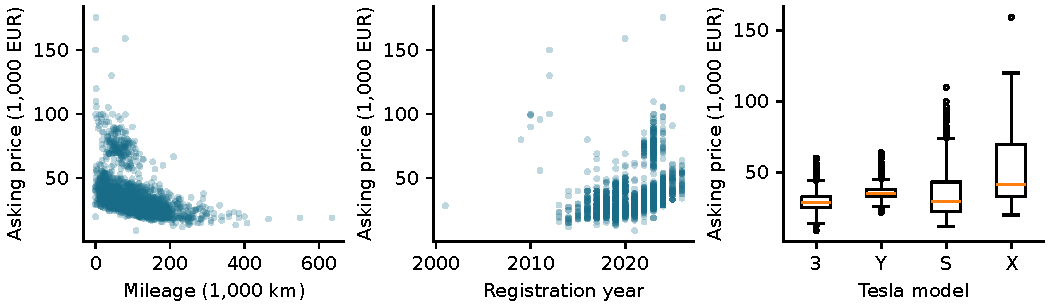
\includegraphics[width=\textwidth]{figures/eda.pdf}
\caption{Training-only price against mileage, first-registration year and Tesla model ($n=3,002$). Units are shown on every axis. Scatterplots retain extremes; boxes show quartiles, with 1.5-IQR whiskers. Association is not a causal depreciation estimate.}
\label{fig:eda}
\end{figure*}

Univariate numeric $r^2$ and categorical correlation ratio $\eta^2$ place power, model, mileage, year and country above equipment and assistance. These common-scale scores use raw EUR price, not log-price. We test three explicit hypotheses: \textbf{H1}, trim indicators reduce error conditional on structured fields; \textbf{H2}, model-specific year interactions improve on a shared slope; \textbf{H3}, these two groups outperform raw correlation ranking. Their verdicts come from matched ablations in Section 7 and coefficient interpretation in Section 8, not from these plots alone.

\section{Method}
\subsection{Pipeline and feature groups}
Figure~\ref{fig:pipeline} traces each listing from raw fields to a EUR prediction.
\begin{figure}[h]
\centering
\fbox{\parbox{.90\columnwidth}{\centering
Advertisement: structured fields + title\\$\downarrow$\\
Parse six keyword flags; form three model $\times$ year terms\\$\downarrow$\\
Training-fold scaling + category vocabulary\\$\downarrow$\\
OLS: standardized representation $\rightarrow$ EUR price\\$\downarrow$\\
Fixed validation/test rows $\rightarrow$ MAE, RMSE, $R^2$}}
\caption{Prediction pipeline. Every learned transformation uses only its fit partition. The target enters regression fitting and evaluation, never feature construction.}
\label{fig:pipeline}
\end{figure}
\textbf{Set A} contains the seven structured fields. \textbf{Set B} retains the top $k$ fields ranked inside each training fold: squared Pearson correlation for numeric fields and between-category/total target sum of squares for nominal fields. Searching $k=1,\ldots,7$, the smallest value within one standard error ($s/\sqrt{5}$) of the lowest CV MAE is $k=\SelectedK{}$, favoring a smaller representation when gains are within fold uncertainty.

\textbf{Set C}, our final OLS representation, keeps all seven raw fields and adds two groups. Six case-insensitive title flags mark Performance/Plaid, Long Range, AWD/Dual Motor, entry trim (RWD/Standard Range), new generation (Highland/Juniper/Plaid/refresh) and HW4. These capture within-model differences that power alone may miss (H1). Flags are mentions, not verified configurations: Plaid activates two flags, and Standard Range does not certify rear-wheel drive. The reproducibility package preserves exact expressions.

Three interactions allow Model S, X and Y to have different registration slopes:
\begin{equation}
u_m=\mathbf{1}(\mathrm{model}=m)(\mathrm{year}-\overline{\mathrm{year}}_{\mathrm{fit}}).
\end{equation}
They address H2. The fit-partition mean prevents validation-dependent centering. Model 3 shares the base slope with rare models; these latter classes cannot support reliable separate slopes. This is a registration-year association, not observed longitudinal depreciation.

\subsection{Linear model and alternatives}
OLS minimizes $\sum_i(y_i-b-\mathbf z_i^T\boldsymbol\beta)^2$. It offers direct EUR effects and a small fixed representation, while interactions allow non-additive raw-input behavior. It has no regularization parameter. No target logarithm, post-hoc clipping or higher-order polynomial search is used. Full one-hot fitting uses a least-squares solution; inference uses an equivalent full-rank reference coding. The retained representation has \NumParameters{} coefficients including the intercept.

Ridge is a plausible alternative for correlated features. A training-only dealer-grouped sensitivity searches $\alpha\in\{.01,.1,1,10,100,1000\}$ on the same Set C inputs; the lowest MAE is \eur\RidgeBest{} at $\alpha=\RidgeAlpha{}$, compared with OLS \eur\GroupC{}. We retain the already specified OLS benchmark and report this alternative without choosing a new model from test outcomes. Coefficient uncertainty is conditional on this representation.

\section{Experimental Setup}
\subsection{Validation and provenance}
We use identical five-fold shuffled KFold partitions (seed 42) across methods, plus five-fold GroupKFold by seller/dealer as the structure-aware check. Five folds retain about 80\% for fitting while permitting a spread estimate at modest cost. There are \TrainGroups{} training dealer groups; each missing seller receives its own group. Scaling, encoding, centering and top-$k$ ranking are fitted within folds. We report mean $\pm$ sample SD. Feature-set/k exploration used these training folds, so CV is development evidence, not a nested estimate of the entire selection process.

The supplied test set was already inspected in earlier team analyses. We freeze this integration's model definitions before recomputation and retain all 752 rows, but do not claim a new one-use blind holdout. Dealer grouping is not a vehicle-identity guarantee; overlap and sensitivity checks are reported separately. A newly collected locked test set remains necessary for confirmatory deployment claims.

\subsection{Metrics and baselines}
MAE measures typical absolute EUR error; RMSE penalizes large misses, and $R^2$ describes explained variation. We propose MAE $\leq$ \eur3,000 as a screening-use threshold, not a validated stakeholder tolerance or an individual guarantee. We also report the proportion of cars within \eur3,000.

Baselines are the \textbf{Trivial Baseline (training mean)}, \textbf{Simple Baseline (mileage-only OLS)}, and \textbf{Strong Baseline (200-tree random forest on Set A, seed 42; no depth limit, default leaf size 1)}. The forest is an inherited fixed flexible comparator, not a tuned optimum. All methods use identical rows and metrics. Paired test-loss gaps use 10,000 dealer-cluster bootstrap resamples (seed 42), keeping both methods' predictions together. Grouped-fold paired $t$-tests have only five overlapping training fits, so their $p$-values are exploratory.

\section{Results}
\subsection{Main comparison}
\begin{table}[h!]
\centering\small\setlength{\tabcolsep}{3pt}
\begin{tabular}{lrrrr}
\toprule
Method & Group MAE & Test MAE & RMSE & $R^2$\\
\midrule
Mean & 8,552 $\pm$ 1,354 & 8,906 & 14,040 & -0.004\\
Mileage & 7,806 $\pm$ 1,171 & 8,116 & 12,909 & 0.152\\
RF (raw) & \textbf{2,660} $\pm$ \textbf{236} & \textbf{3,227} & \textbf{5,103} & \textbf{0.867}\\
OLS A & 3,991 $\pm$ 429 & 4,290 & 5,971 & 0.818\\
OLS C (ours) & 3,324 $\pm$ 267 & 3,711 & 5,399 & 0.852\\
\bottomrule
\end{tabular}
\caption{Main results: errors in EUR; Group MAE is five-fold mean $\pm$ sample SD. RMSE and $R^2$ use all 752 test rows. Bold marks the best values.}
\label{tab:results}
\end{table}

Table~\ref{tab:results} shows that engineered OLS improves over raw OLS but remains behind the random forest. Test MAE falls by \eur\GainAC{} (\GainPct{}\%) from A to C; the forest's advantage over C is \eur\GapRF{}. A piecewise tree ensemble can capture local trim/usage combinations beyond the three slopes and six flags, although the comparison does not isolate that mechanism. The forest remains a baseline; our final predictor is linear.

Against the proposed threshold, C exceeds \eur3,000 by \eur\ExcessC{}, and RF exceeds it by \eur\ExcessRF{}. Only \WithinC{}\% of C's test errors lie within \eur3,000 (RF: \WithinRF{}\%). The average threshold is not satisfied even though many individual estimates fall inside it. Thus these predictions are inspection aids, not autonomous pricing decisions.

\subsection{Ablations and uncertainty}
\begin{table}[h!]
\centering\small\setlength{\tabcolsep}{3pt}
\begin{tabular}{lrrr}
\toprule
Set & KFold MAE & Group MAE & Test MAE\\
\midrule
A: raw & 3,939 $\pm$ 105 & 3,991 $\pm$ 429 & 4,290\\
B: top-5 & 3,966 $\pm$ 118 & 4,022 $\pm$ 446 & 4,329\\
\textbf{C: full} & 3,244 $\pm$ 92 & 3,324 $\pm$ 267 & 3,711\\
C $-$ flags & 3,457 $\pm$ 95 & 3,522 $\pm$ 278 & 3,871\\
C $-$ interactions & 3,705 $\pm$ 58 & 3,779 $\pm$ 414 & 4,081\\
\bottomrule
\end{tabular}
\caption{Matched OLS ablations, EUR. All folds and preprocessing rules are shared. Lower is better; C is best in every column.}
\label{tab:abl}
\end{table}

Only the feature representation changes in Table~\ref{tab:abl}; every row uses OLS and the same splits. Removing either engineered group worsens dealer-grouped CV, supporting H1 and H2. Set C also improves on top-$k$ Set B, supporting H3: ranking raw associations cannot create title information or model-specific slopes. Both groups use already collected fields, adding nine numeric terms rather than a new data source. Their costs are parsing maintenance and harder interpretation of overlapping trim mentions.

\begin{table}[h!]
\centering\small\setlength{\tabcolsep}{3pt}
\begin{tabular}{lrrr}
\toprule
Comparison & Gap & 95\% cluster CI & $p$\\
\midrule
A $-$ C & 578 & [374, 796] & 0.001\\
B $-$ C & 617 & [407, 844] & 0.002\\
RF $-$ C & -484 & [-752, -205] & 0.001\\
\bottomrule
\end{tabular}
\caption{Test-MAE gaps (EUR): positive favors C. CI: paired dealer-cluster bootstrap, 10,000 draws; $p$: exploratory paired grouped-fold $t$-test.}
\label{tab:gaps}
\end{table}

The paired bootstrap intervals in Table~\ref{tab:gaps} preserve within-dealer dependence in test losses. They describe uncertainty for these fixed fitted models and observed sellers; they omit retraining, feature selection and market change. Reused test data and uncertain vehicle identity prevent treating these intervals as definitive prospective evidence.

\begin{table}[h!]
\centering\fontsize{8}{9.5}\selectfont\setlength{\tabcolsep}{1.6pt}
\begin{tabular}{lrrrrrrr}
\toprule
Model & $n$ & A & B & C & Gain & Med. & $\leq$3k\\
\midrule
3 & 347 & 3,467 & 3,481 & 3,004 & -13\% & 7.9\% & 63\%\\
S & 69 & 6,790 & 6,917 & 6,289 & -7\% & 16.7\% & 29\%\\
Y & 271 & 3,723 & 3,770 & 3,161 & -15\% & 6.7\% & 58\%\\
X & 59 & 7,816 & 7,876 & 6,423 & -18\% & 9.5\% & 42\%\\
Roadster & 5 & 12,403 & 12,395 & 11,976 & -3\% & 13.0\% & 0\%\\
Cybertruck & 1 & 22,051 & 21,858 & 19,203 & -13\% & 12.0\% & 0\%\\
All & 752 & 4,290 & 4,329 & 3,711 & -13\% & 8.0\% & 56\%\\
\bottomrule
\end{tabular}
\caption{Test MAE (EUR). Gain $=100(C/A-1)\%$; negative means lower error. Med.: C median absolute percentage error; $\leq$3k: share within EUR 3,000. All aggregates all 752 cars; rare classes are not interpreted.}
\label{tab:slices}
\end{table}

Table~\ref{tab:slices} shows how gains vary by model. Larger absolute errors for S/X can reflect heterogeneous trims and price scales, not simply worse percentage accuracy. Rare classes must not be interpreted from their tiny sample sizes. The same representation can improve common-model averages while remaining unreliable on individual outliers.

\paragraph{Sensitivity to data quality.}
A model/registration-month/mileage duplicate proxy flags \OverlapN{} test rows overlapping training. On the \NonoverlapN{} remaining rows, MAE is \eur\NonoverlapA{} (A), \eur\NonoverlapC{} (C), and \eur\NonoverlapRF{} (RF). Matching attributes do not prove identical vehicles; exclusion is a sensitivity analysis, not a replacement split. Removing the single Model Y/2001 training record and refitting C gives test MAE \eur\SuspectMAE{}. This post-hoc audit is not used to optimize the headline model.

\section{Analysis}
\subsection{Coefficients and significance}
\begin{table}[h!]
\centering\small\setlength{\tabcolsep}{3pt}
\begin{tabular}{lrrrr}
\toprule
Term & $\beta$ & 95\% CI & $p$ & VIF\\
\midrule
Year & 4.56 & [4.01, 5.12] & $<.001$ & 5.9\\
Mileage & -3.44 & [-3.90, -2.98] & $<.001$ & 1.7\\
Power & 2.78 & [2.31, 3.25] & $<.001$ & 3.4\\
Equipment & 0.19 & [-0.03, 0.41] & 0.097 & 1.3\\
Performance & 1.19 & [0.88, 1.50] & $<.001$ & 2.1\\
Long range & 0.53 & [0.18, 0.87] & 0.003 & 2.0\\
AWD & -0.73 & [-1.14, -0.32] & $<.001$ & 2.4\\
Entry trim & -0.61 & [-0.91, -0.30] & $<.001$ & 2.9\\
New gen. & 1.02 & [0.76, 1.29] & $<.001$ & 1.4\\
HW4 & 0.74 & [0.47, 1.01] & $<.001$ & 1.1\\
Model S$\times$year & 3.17 & [2.61, 3.74] & $<.001$ & 4.2\\
Model X$\times$year & 2.96 & [2.34, 3.58] & $<.001$ & 2.4\\
Model Y$\times$year & -0.27 & [-1.54, 0.99] & 0.675 & 2.7\\
Cybertruck & 133.40 & --- & --- & 1.0\\
Model S & 20.31 & [18.81, 21.81] & $<.001$ & 3.5\\
Model X & 24.76 & [22.81, 26.71] & $<.001$ & 2.5\\
Model Y & 3.24 & [1.24, 5.24] & 0.002 & 2.3\\
Roadster & 85.02 & [65.55, 104.50] & $<.001$ & 1.5\\
Unknown & -11.69 & [-28.99, 5.61] & 0.185 & 1.0\\
AT & -0.09 & [-0.77, 0.59] & 0.790 & 1.3\\
DE & -0.39 & [-1.02, 0.24] & 0.221 & 1.7\\
BE & -0.84 & [-1.59, -0.09] & 0.028 & 1.3\\
FR & -0.29 & [-1.23, 0.66] & 0.550 & 1.2\\
LU & -0.10 & [-3.19, 3.00] & 0.950 & 1.0\\
IT & 2.78 & [2.08, 3.47] & $<.001$ & 1.5\\
ES & -1.43 & [-2.23, -0.63] & $<.001$ & 1.3\\
EAP & 0.60 & [-0.35, 1.54] & 0.214 & 1.0\\
FSD & 0.87 & [0.13, 1.61] & 0.022 & 1.1\\
\bottomrule
\end{tabular}
\caption{Final Set C coefficients and HC3 intervals in 1,000 EUR. Standardized numeric terms, reference-coded category contrasts; all 28 non-intercept terms shown. Cybertruck ($n=1$): uncertainty unavailable. Model contrasts apply at the training mean year.}
\label{tab:coef}
\end{table}

Table~\ref{tab:coef} covers all non-intercept terms in the final Set C model, including rare categories. Numeric inputs, binary flags and interaction products are standardized before fitting; their effects are EUR per training SD. Category contrasts use Model 3, Netherlands and AP as references and remain 0/1. For a flag, divide its standardized coefficient by its SD to obtain a 0-to-1 premium. No coefficient is a percentage change, because the target is not logged.

Intervals and two-sided $p$-values use HC3 heteroskedasticity-robust OLS $t$ inference. The single training Cybertruck has unit leverage: its own coefficient's interval is not identifiable. We report its fitted effect but mark interval and $p$ unavailable; other intervals come from the algebraically equivalent fit excluding that singleton row and dummy. This avoids presenting a numerical artifact as evidence. HC3 does not correct dealer dependence; inferential results are conditional, exploratory associations, with no multiple-testing correction. VIF uses the full-rank design including an intercept.

\paragraph{Interpretation.} Each newer year adds EUR 1,882 for Model 3, about EUR 4,178 for S and EUR 4,994 for X; Y does not differ significantly. Mileage adds EUR $-590$ per 10,000 km; power adds EUR 220 per 10 kW. Equipment adds EUR 9/item, not significantly. These are conditional associations, not causal depreciation. HW4, new generation, Performance and Long Range carry premiums; entry trim a discount. Italy (+EUR 2,775), Spain ($-$1,430) and Belgium ($-$842) differ from the Netherlands; other countries do not. FSD adds EUR 866; EAP is not significant.

AWD ($-$EUR 1,461) overlaps other terms: 88\% of flagged listings carry Long Range or Performance, with more power (318 vs 282 kW). A Performance AWD car nets +EUR 1,480. Raw AWD listings are also cheaper (EUR 34,596 vs 36,016), so the sign is not a reversal. These overlap summaries follow the team\textquotesingle s revised analysis.

\paragraph{Resolving the hypotheses.}
H1 and H2 are predictive group hypotheses, so the relevant tests are removals in Table~\ref{tab:abl}, not whether every flag or interaction separately has $p<.05$. H3 is resolved by C versus B in Tables~\ref{tab:abl} and \ref{tab:gaps}. A small $p$-value does not make an effect useful: compare its natural-unit size to the \eur3,000 screening tolerance. Conversely, a sparse feature can have a wide interval while the combined group improves validation MAE. Shared trim words, model mix and omitted battery condition offer alternative explanations to causal premiums.

\subsection{Error analysis}
\begin{table}[h!]
\centering\small\setlength{\tabcolsep}{3pt}
\begin{tabular}{lrrr}
\toprule
Case & Actual & Predicted & Error\\
\midrule
1 & 75,900 & 34,842 & 41,058\\
2 & 90,000 & 61,820 & 28,180\\
3 & 12,000 & -15,506 & 27,506\\
\bottomrule
\end{tabular}
\caption{Three largest absolute errors of final Set C (EUR). Error = actual $-$ predicted; context and explanations below.}
\label{tab:cases}
\end{table}

\begin{figure}[h]
\centering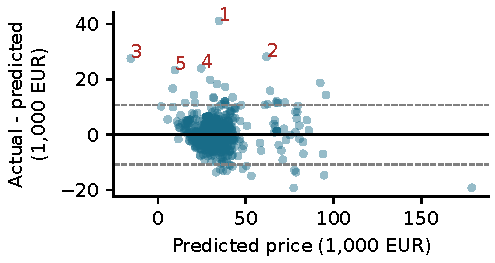
\includegraphics[width=\columnwidth]{figures/residuals.pdf}
\caption{Set C test residuals, actual minus predicted EUR. Labels mark the three largest absolute errors in Table~\ref{tab:cases}; all 752 test rows are shown.}
\label{fig:resid}
\end{figure}
\textbf{Case 1:} Model X 75D Dual Motor, France, 2018, 49,931 km, 193 kW. The EUR 75,900 advertisement is far above its estimate. A training-only comparison finds 27 comparable 2017--2019 Model X ``75 training listings with median EUR 27,900 and maximum EUR 39,999. Unobserved condition or unusual pricing is plausible; an error cannot prove mispricing.

\textbf{Case 2:} Model X ``75 kWh Dual Motor, Belgium, 2023, 32,000 km, 244 kW. The high asking price and registration year conflict with the older-looking title. Incorrect metadata or an unobserved configuration could explain the miss; neither is independently verified.

\textbf{Case 3:} Model S 85 Base, Netherlands, 2014, 670,000 km, 300 kW. Mileage exceeds the training maximum of 635,000 km. The linear extrapolation produces EUR $-15,506$, despite an actual EUR 12,000. This is a model failure, not just noisy labels. C produces one negative test prediction. The shared underprediction pattern in Figure~\ref{fig:resid} motivates input-consistency and coverage flags first; validated battery condition and a new held-out evaluation should precede any automatic correction.

\section{Conclusion and Limitations}
Title indicators and model-specific registration slopes improve this linear benchmark: test MAE is \eur\TestC{}, versus \eur\TestA{} for raw OLS and \eur\TestRF{} for RF. Ablations support both engineered groups and improvement over raw correlation ranking. The gain is useful but insufficient for the proposed \eur3,000 average-error threshold. Buyers should use the estimate to prioritize inspections and verify trim, battery condition and anomalous specifications before negotiating.

Coverage is one website, eight countries and one snapshot of asking prices. The supplied order split, prior test exposure, possible duplicate cars, inherited annotations, rare classes and uncertain seller measurements limit generalization. The threshold is an assumed fixed EUR cost and is relatively stricter on cheaper cars. Linear extrapolation can be implausible; fitted associations are not causal depreciation. The next experiment should freeze these rules, collect a new locked snapshot with vehicle-identity and battery-condition checks, and evaluate both price accuracy and actual screening decisions.

\section*{Contributions of Each Member}
Responsibilities were shared within each subgroup. \textbf{A}: abstract, problem formulation, literature, data collection/preprocessing, EDA and feature pipeline (Sections 1--5.1; Figures 1--2). \textbf{B}: model choice/tuning, validation, metrics, threshold, baselines and main comparisons with significance testing (Sections 5.2--7.1). \textbf{C}: ablations, coefficients/significance/VIF, error cases and conclusions (Sections 7.2--9; Figure 3).
\ifdefined\judgeversion
\begin{itemize}\setlength\itemsep{0pt}
\item Member 1: Group A responsibilities above.
\item Member 2: Group B responsibilities above.
\item Member 3: Group B responsibilities above.
\item Member 4: Group A responsibilities above.
\item Member 5: Group C responsibilities above.
\item Member 6: Group C responsibilities above.
\item Member 7: Group B responsibilities above.
\end{itemize}
\else
\begin{itemize}\setlength\itemsep{0pt}
\item \cn{馮昱祥} (515559007): Group A tasks above.
\item \cn{邱育宏} (315554053): Group B tasks above.
\item \cn{吳宥駒} (315551146): Group B tasks above.
\item \cn{林暉庭} (314551160): Group A tasks above.
\item \cn{黃少鋒} (315561001): Group C tasks above.
\item \cn{莊誌強} (315561002): Group C tasks above.
\item \cn{杜洺鋒} (315554001): Group B tasks above.
\end{itemize}
\fi
\paragraph{AI usage.} ChatGPT/Codex assisted with code revision, experimental recomputation, plots, literature checking, writing and compilation. Team packages supplied the data and feature definitions; the team retains responsibility for verifying the integrated results.
\bibliography{references}
\end{document}
